\chapter{Mordente}

Tras estudiar la motivación de este trabajo y habiendo justificado la necesidad de una alternativa software para la gestión de agrupaciones musicales, pasamos a desarrollar el producto.

Para esta fase se va a hacer uso de la llamada metodología de Diseño Centrado en el Usuario (UCD por sus siglas en inglés), descrita en el siguiente apartado. 

\section{Desarrollo de Mordente}

En este punto se van a establecer las metodologías de diseño a seguir durante el desarrollo de la herramienta, de modo que tengamos disponibles unas guías a seguir durante el proceso y unas herramientas que nos permitan definir la funcionalidad esperada y concretar las necesidades de los futuros usuarios.

\subsection{Diseño Centrado en el Usuario}

El Diseño Centrado en el Usuario está estrechamente relacionado con el Diseño Centrado en el Humano\cite{w3UCD}. Este último ``es una aproximación al desarrollo de sistemas interactivos que se centra específicamente en hacer sistemas usables. Es una actividad multi-disciplinar.''\cite{isoHCD}.

Los principios\cite{jeffreyUCD} en los que se fundamenta se pueden resumir en:

\begin{enumerate}
    \item \textbf{Aproximación temprana a usuarios y tareas}: la recogida de información es estructurada y sistemática.
    \item \textbf{Medida empírica y testeo del uso del producto}: se centra en la facilidad de aprendizaje y de uso, y la prueba de prototipos con usuarios reales.
    \item \textbf{Diseño iterativo}: el producto se diseña, modifica y prueba de forma repetida, permitiendo repensar completamente la idea gracias a la prueba de modelos conceptuales tempranos.
\end{enumerate}

\subsection{Design Thinking}

El Design Thinking es un proceso de diseño descrito en cinco fases:\cite{designThinkingPlattner} definir el problema, buscar las necesidades, idear, construir y probar. Este proceso nos ayuda a aplicar el Diseño Centrado en el Usuario mediante una serie de procesos.

\subsubsection{Procesos}

Otros autores hablan de que el Design Thinking no se compone de fases sino de varios espacios que no son secuenciales: se solapan y se forma un bucle entre ellos, repitiéndolo más de una vez y explorando distintas aproximaciones\cite{designThinkingBrown}.

\begin{enumerate}
    \item \textbf{Inspiración}: se observa cómo funcionan las personas para encontrar problemas y oportunidades.
    \item \textbf{Empatía}: se trata de entender los deseos y necesidades de los potenciales clientes, no solo de forma técnica sino sabiendo por qué hacen las cosas de la forma actual y qué les resulta más importante.
    \item \textbf{Ideación}: se trata de una combinación de pensamiento divergente y convergente. El pensamiento divergente genera nuevas ideas de forma creativa, mientras que el convergente trata de sintetizar las ideas y elegir las mejores.
    Teniendo diversas personas en el equipo, la técnica más utilizada es el \textit{brainstorming}, en el que todos los miembros dan ideas espontáneas que se apuntan de forma que cada nueva idea puede fomentar la creatividad de los demás.
    \item \textbf{Implementación y prototipado}: en este proceso las ideas se convierten en productos concretos. Durante este proceso se van generando diversos prototipos que se prueban con usuarios reales para seguir mejorando la idea.
\end{enumerate}


\section{Personas ficticias}

Las personas ficticias se crean dentro de una técnica perteneciente al Design Thinking. Se tratan de representaciones ficticias de los usuarios, con metas, motivaciones, características y comportamientos de un grupo real de usuarios.\cite{personnas}

Esta técnica nos permite diseñar para personas reales y no para ``usuarios'' abstractos.

En el caso del proyecto que nos ocupa, se han creado cuatro personas ficticias: dos que cumplirían el rol de ``administrador'' en el sistema y otras dos que lo usarían únicamente como miembros.

\begin{figure}[h]
\centering
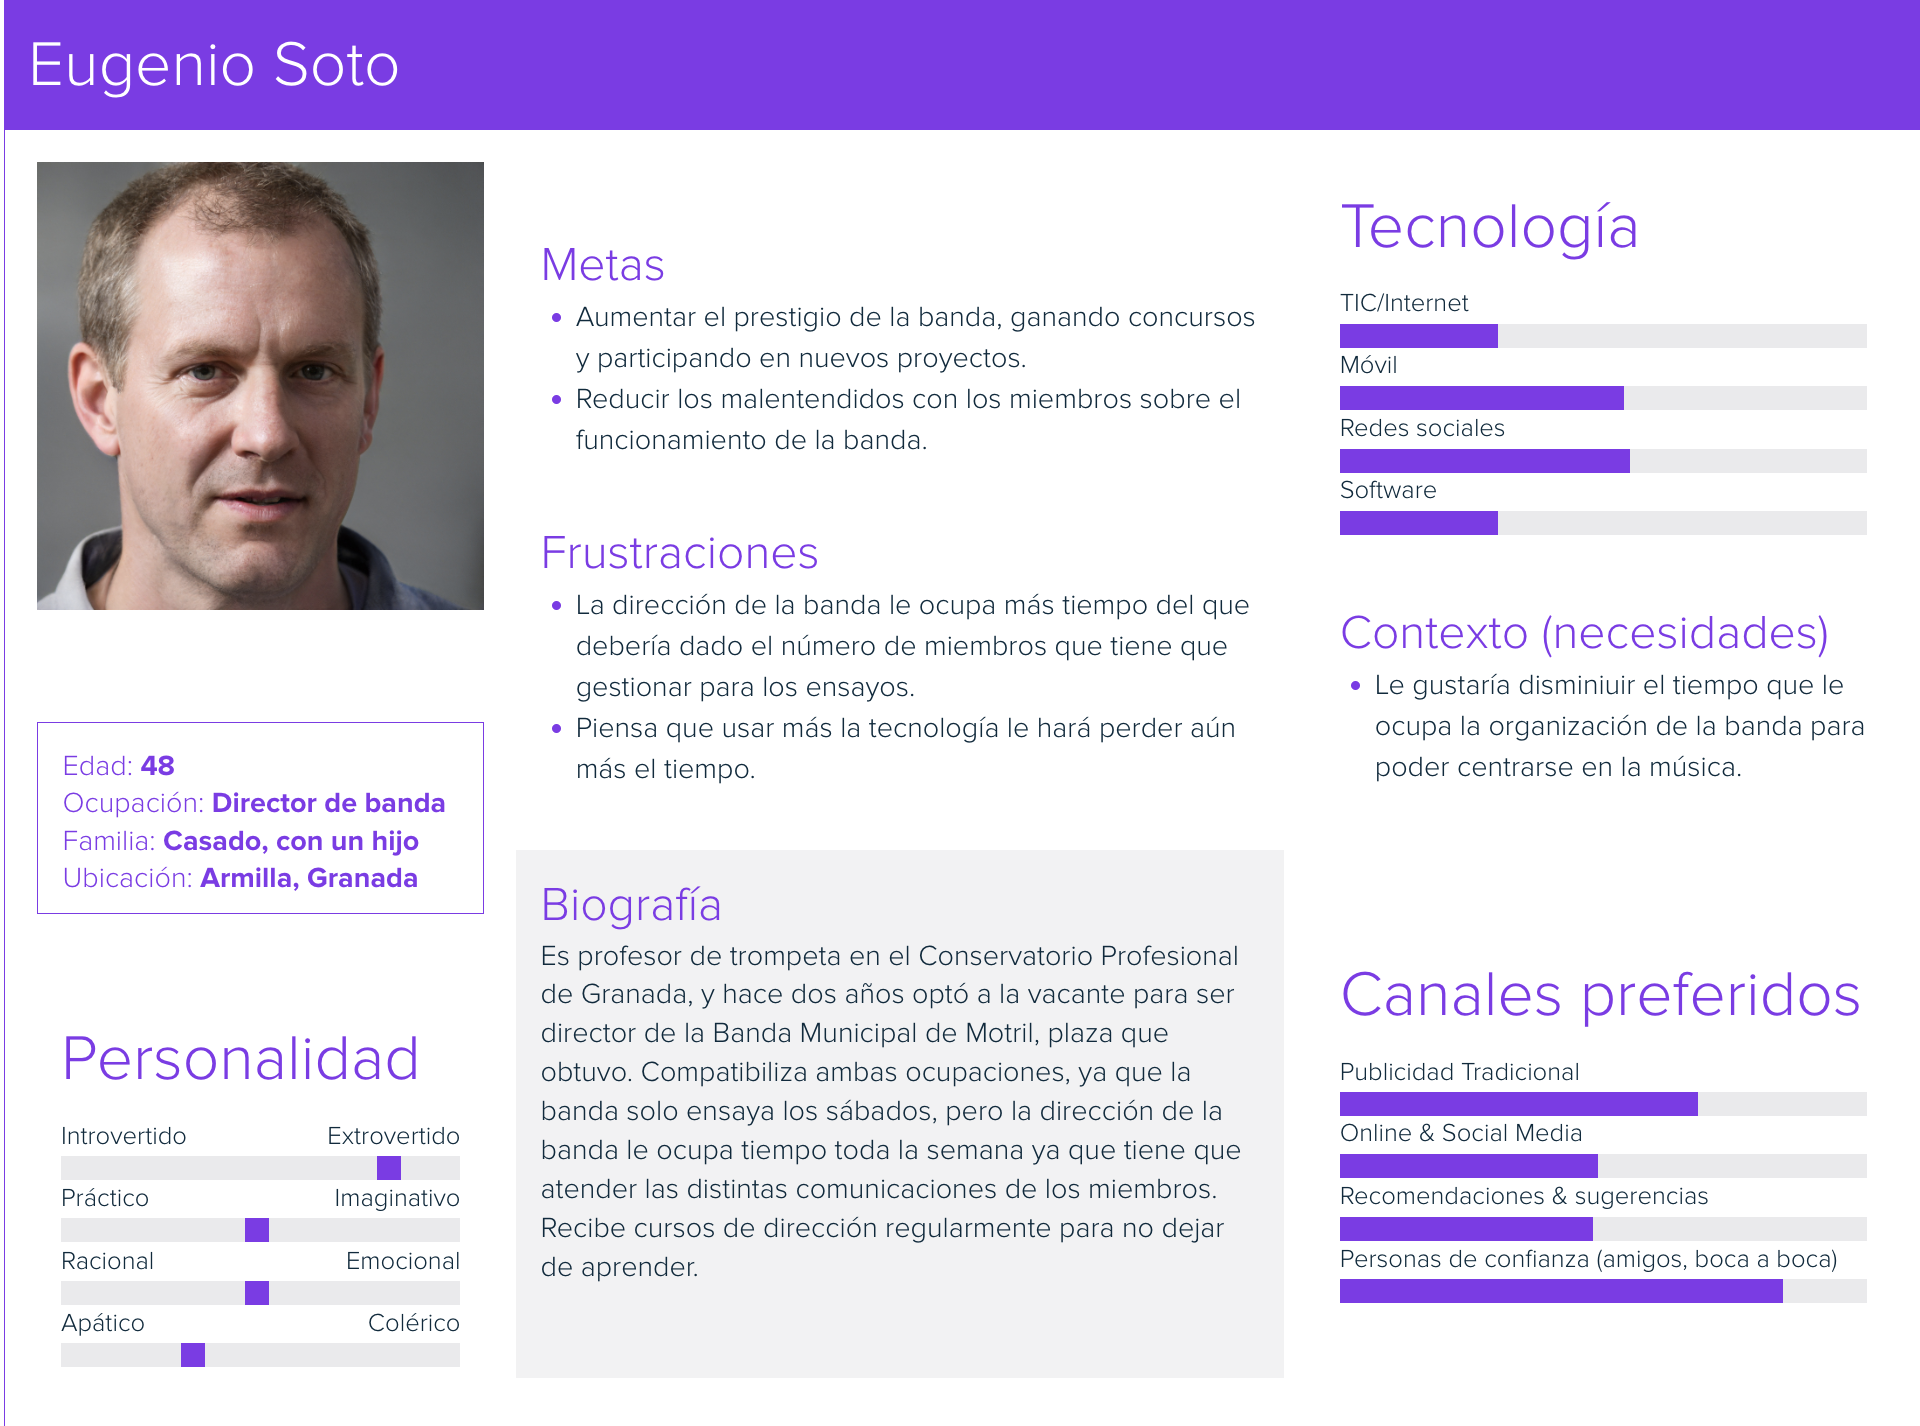
\includegraphics[width=0.8\textwidth]{imagenes/personas/persona_eugenio.png}
\caption{Persona: Eugenio Soto}
\label{fig:persona_eugenio}
\end{figure}

\begin{figure}[h]
\centering
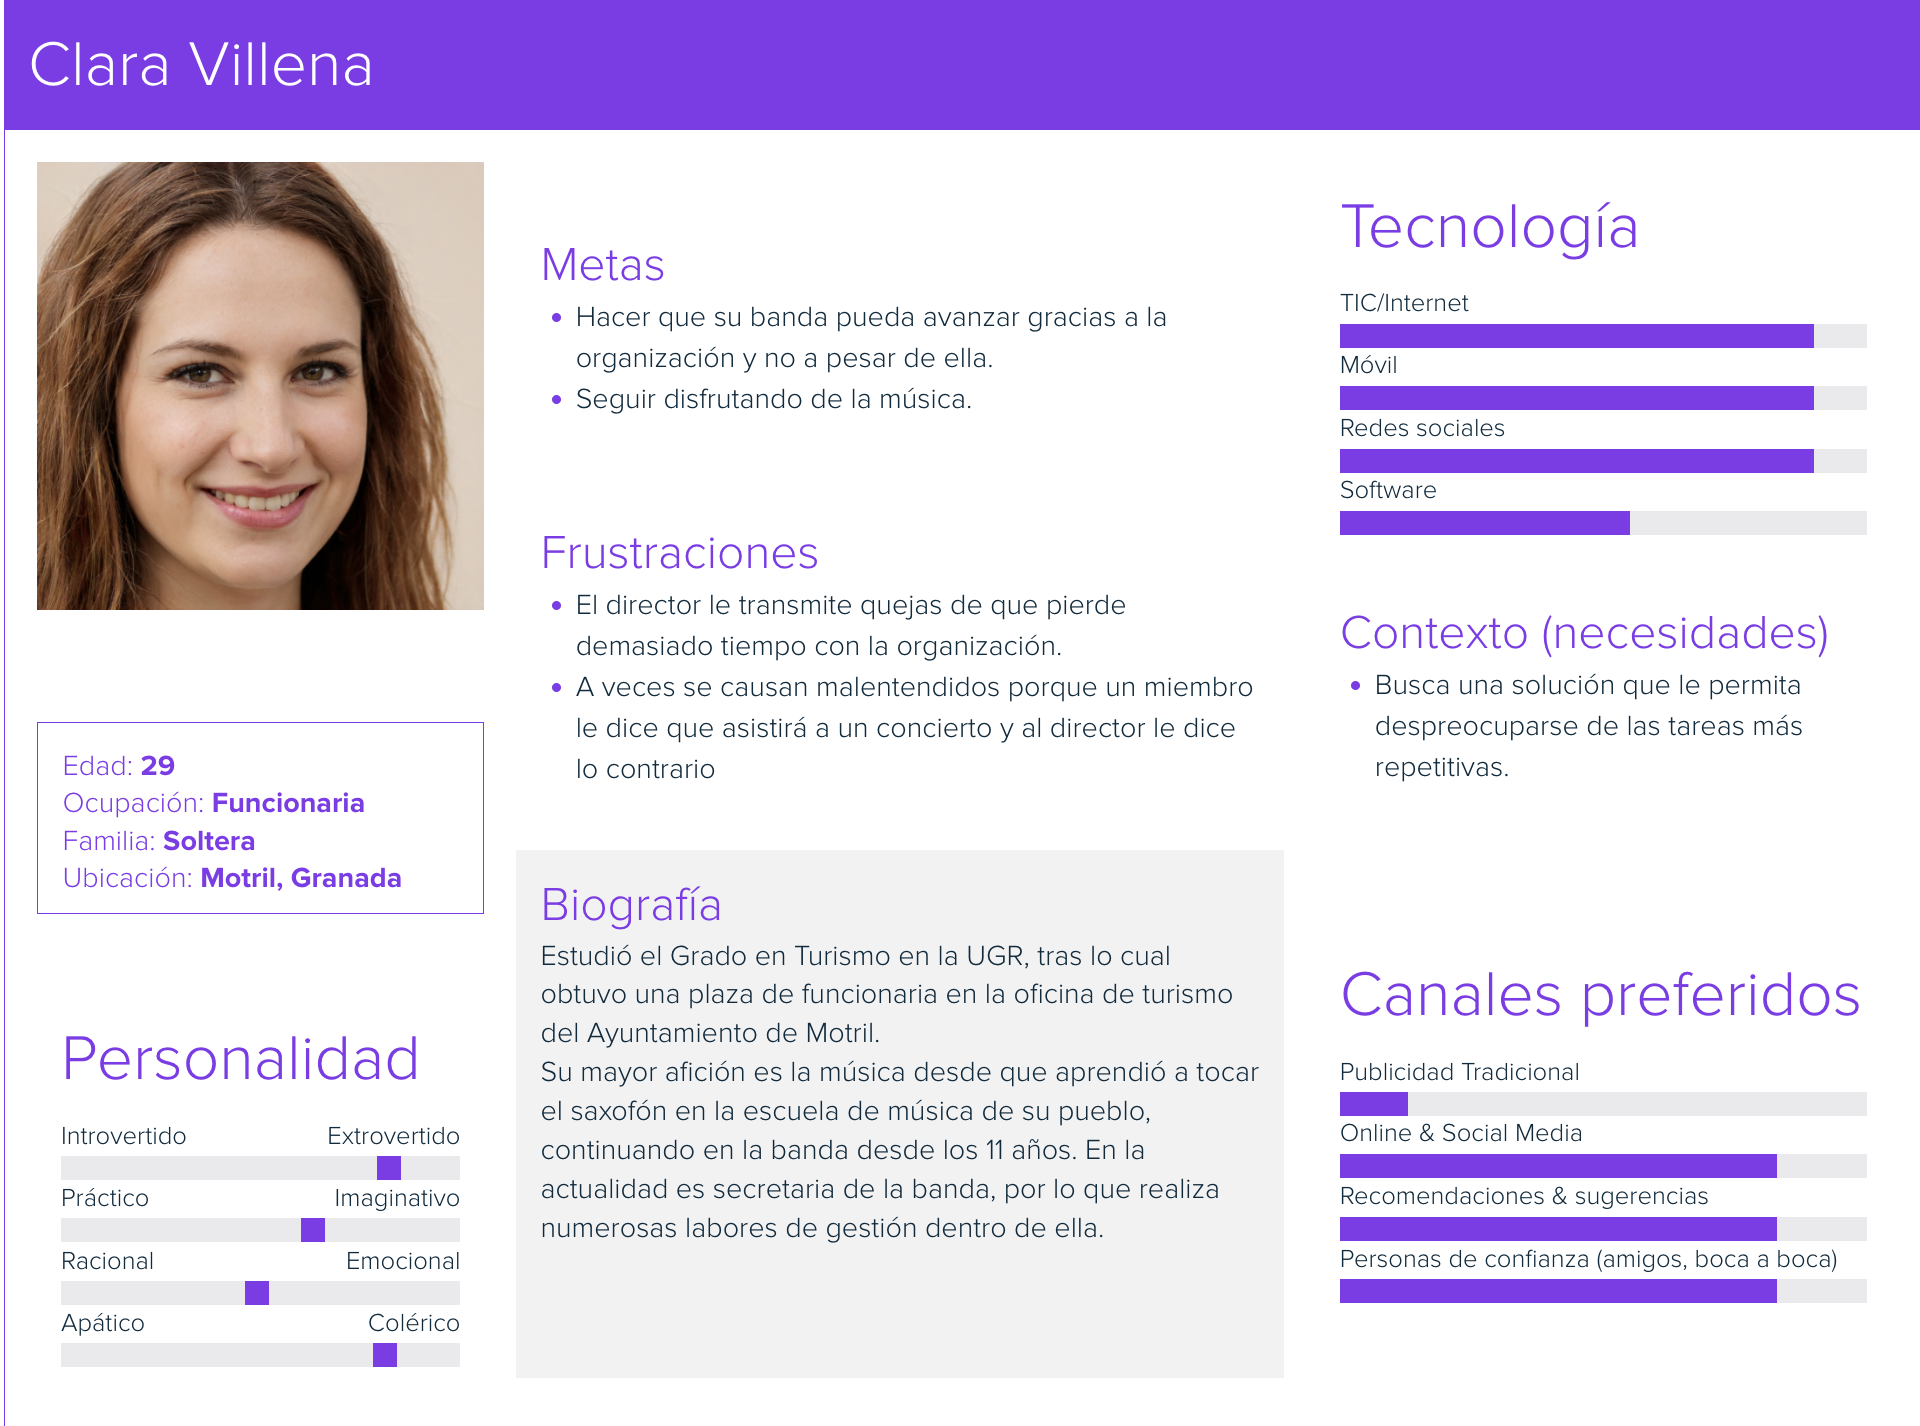
\includegraphics[width=0.8\textwidth]{imagenes/personas/persona_clara.png}
\caption{Persona: Clara Villena}
\label{fig:persona_clara}
\end{figure}


Las figuras \ref{fig:persona_eugenio} y \ref{fig:persona_clara} muestran dos personas que se dedican a la organización de la banda, Eugenio más desde el punto de vista musical y Clara desde el logístico.

Mientras Clara está claramente más familiarizada con las nuevas tecnologías, Eugenio muestra algunas reticencias que deberemos tratar durante el desarrollo, de forma que el producto final sea fácilmente usable y accesible. Igualmente, ya que Clara sí usa las nuevas tecnologías habitualmente, el producto tiene que ser atractivo para ella de forma que no suponga un retroceso con respecto a las herramientas actuales.

Los perfiles que vemos en las figuras \ref{fig:persona_david} y \ref{fig:persona_inma} se refieren a personas que acuden como miembros a la banda de su respectivo pueblo. A Inma se aplican las mismas restricciones que a Eugenio, además de que debemos asegurarnos de que realmente facilitamos que los miembros recuerden los eventos diarios para hacerles la vida más fácil. Con respecto a David, cabe reseñar que, ya que la música no es su mayor afición, preferirá usar la app durante el menor tiempo posible, por lo que se debe intentar que las notificaciones que le lleguen le permitan responder de forma rápida.



\begin{figure}[h]
\centering
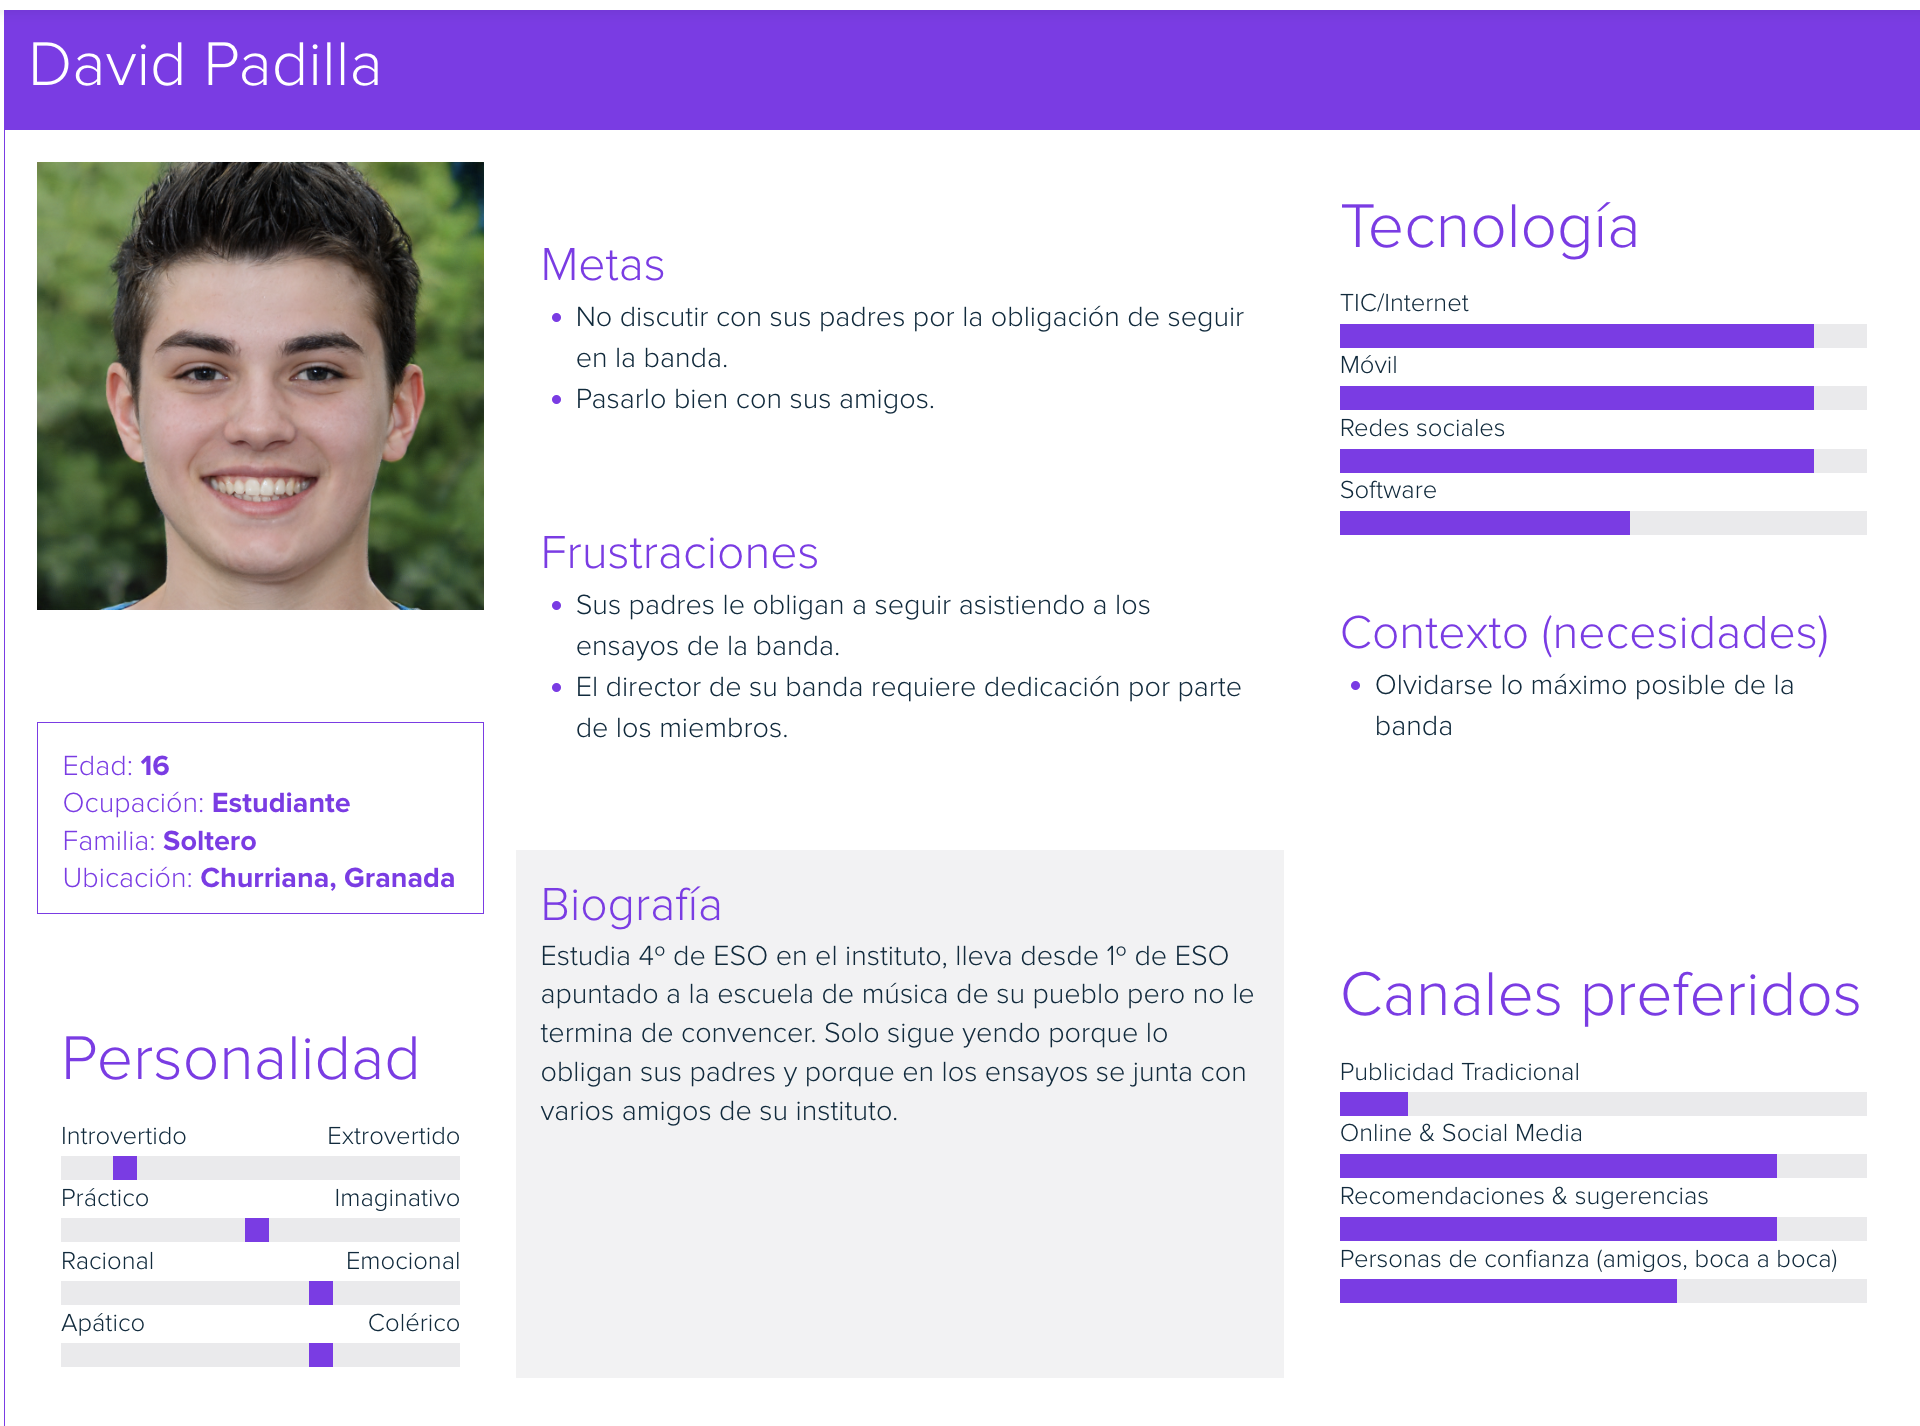
\includegraphics[width=0.8\textwidth]{imagenes/personas/persona_david.png}
\caption{Persona: Eugenio Soto}
\label{fig:persona_david}
\end{figure}

\begin{figure}[h]
\centering
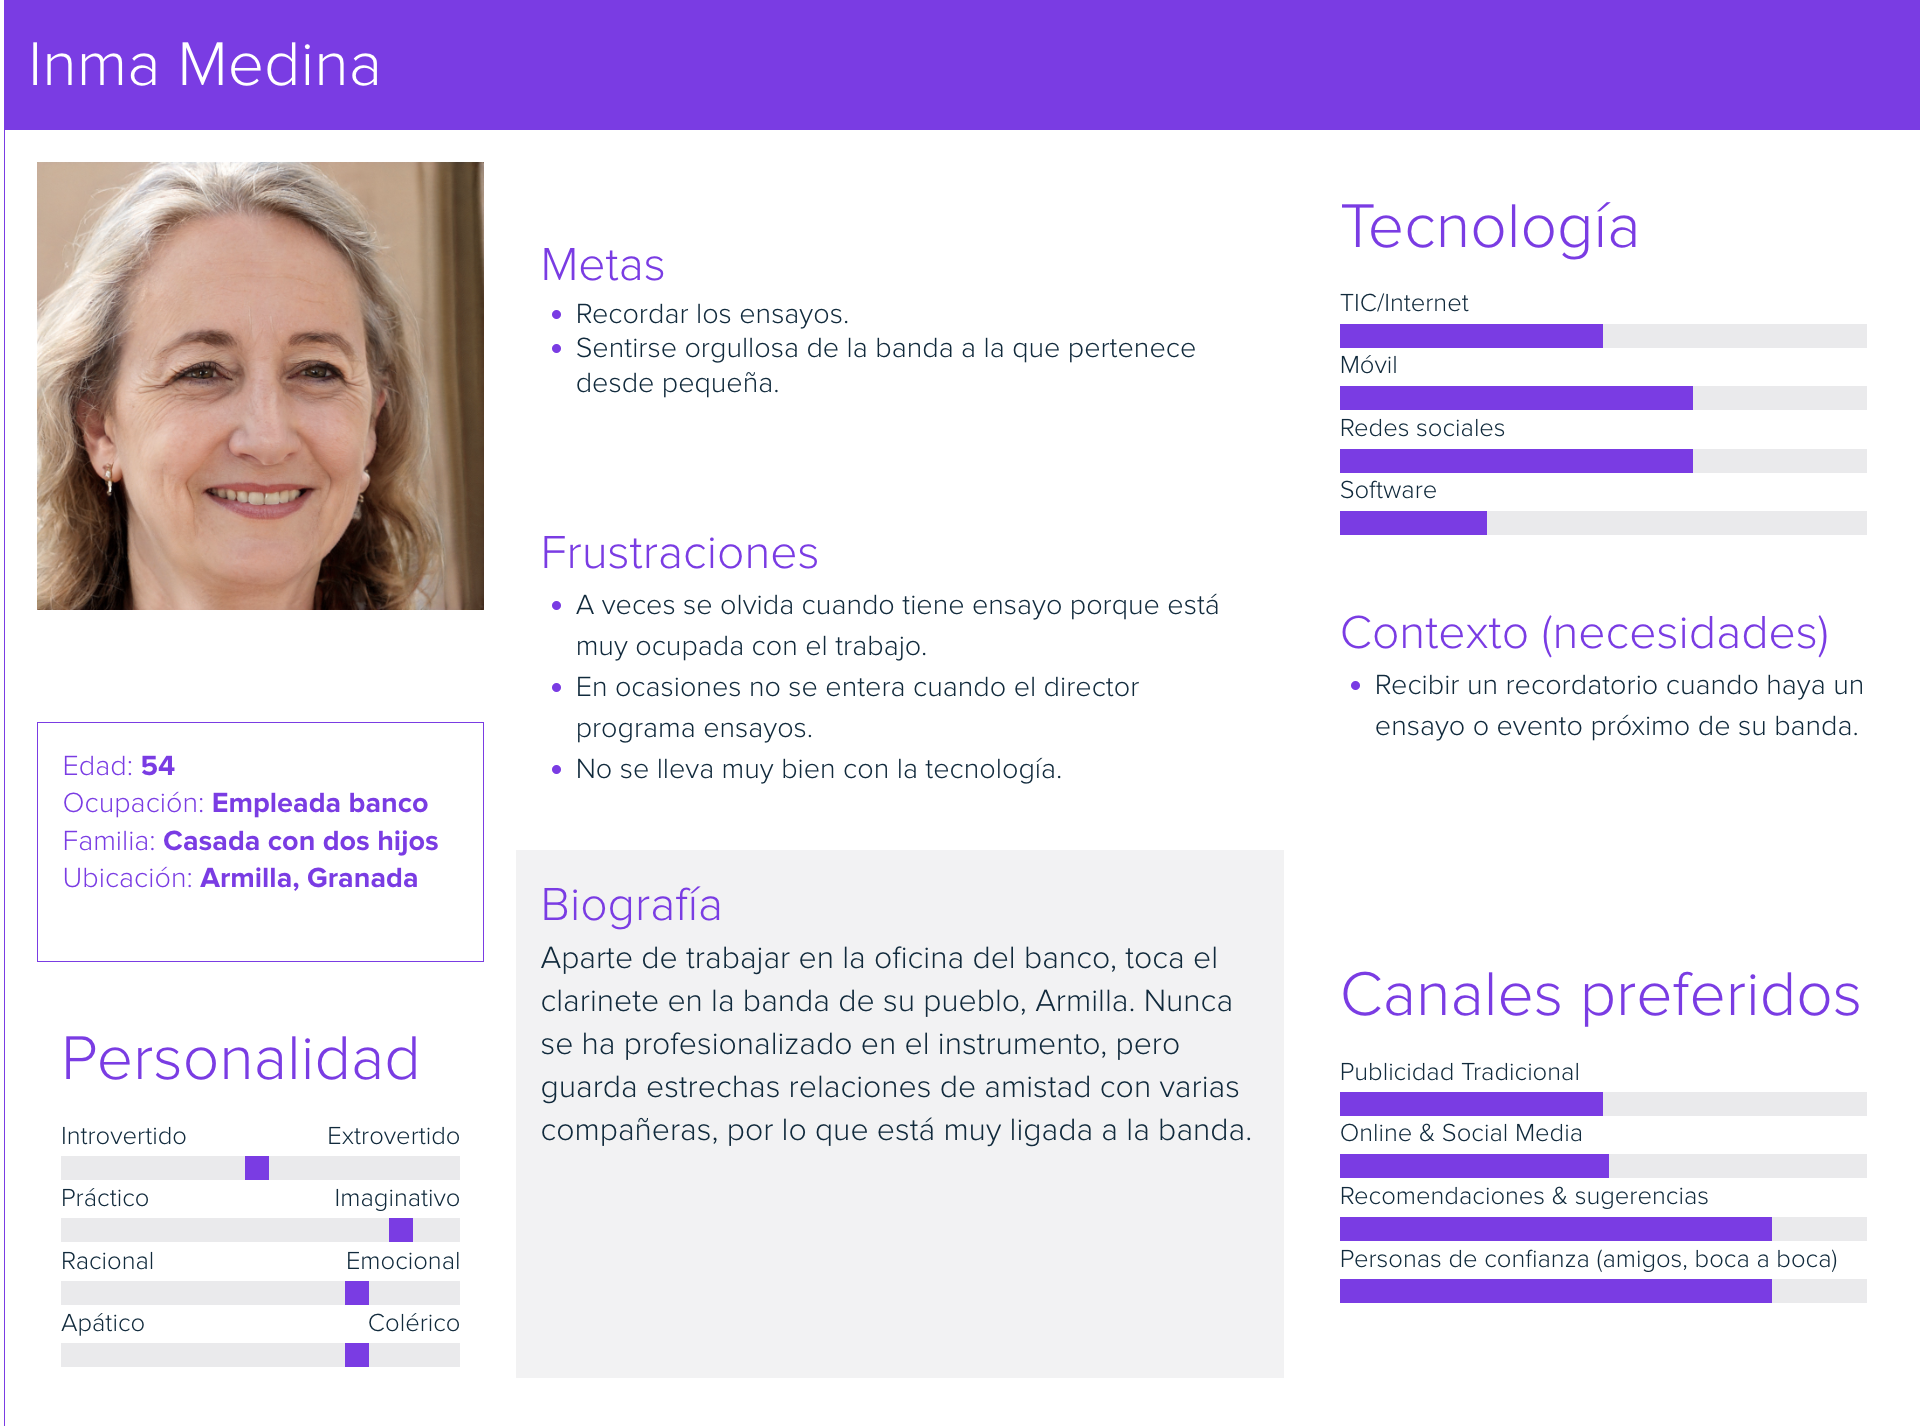
\includegraphics[width=0.8\textwidth]{imagenes/personas/persona_inma.png}
\caption{Persona: Inma Medina}
\label{fig:persona_inma}
\end{figure}

\section{Malla receptora de información}

La malla receptora de información (\textit{Feedback Capture Grid}) 


\subsection{Aspectos interesantes o relevantes de la idea}


\subsection{Críticas constructivas o posibilidades de mejora}


\subsection{Preguntas nuevas a partir de la experiencia del usuario}


\subsection{Ideas que surgen}


\section{Descripción de la propuesta}

\subsection{Propuesta del producto}


\subsection{Elección de metodología de desarrollo}


\subsection{Planificación}


\subsection{Presupuesto}


